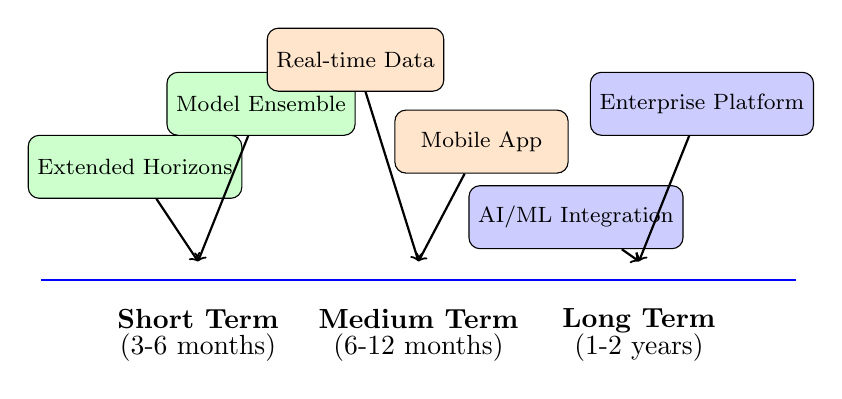
\begin{tikzpicture}[scale=0.8]
	% Timeline - moved up
	\draw[thick, blue] (0,2.5) -- (12,2.5);
	
	% Time periods - moved up
	\node[below] at (2.5,2.2) {\textbf{Short Term}};
	\node[below] at (2.5,1.8) {(3-6 months)};
	\node[below] at (6,2.2) {\textbf{Medium Term}};
	\node[below] at (6,1.8) {(6-12 months)};
	\node[below] at (9.5,2.2) {\textbf{Long Term}};
	\node[below] at (9.5,1.8) {(1-2 years)};
	
	% Short term enhancements - moved up
	\node[rectangle, draw, rounded corners, minimum width=2.2cm, minimum height=0.8cm, 
	align=center, fill=green!20] (short1) at (1.5,4.3) {\footnotesize Extended Horizons};
	\node[rectangle, draw, rounded corners, minimum width=2.2cm, minimum height=0.8cm, 
	align=center, fill=green!20] (short2) at (3.5,5.3) {\footnotesize Model Ensemble};
	
	% Medium term enhancements - moved up
	\node[rectangle, draw, rounded corners, minimum width=2.2cm, minimum height=0.8cm, 
	align=center, fill=orange!20] (med1) at (5,6) {\footnotesize Real-time Data};
	\node[rectangle, draw, rounded corners, minimum width=2.2cm, minimum height=0.8cm, 
	align=center, fill=orange!20] (med2) at (7,4.7) {\footnotesize Mobile App};
	
	% Long term enhancements - moved up
	\node[rectangle, draw, rounded corners, minimum width=2.2cm, minimum height=0.8cm, 
	align=center, fill=blue!20] (long1) at (8.5,3.5) {\footnotesize AI/ML Integration};
	\node[rectangle, draw, rounded corners, minimum width=2.2cm, minimum height=0.8cm, 
	align=center, fill=blue!20] (long2) at (10.5,5.3) {\footnotesize Enterprise Platform};
	
	% Arrows to timeline - adjusted connection points
	\draw[->, thick] (short1) -- (2.5,2.8);
	\draw[->, thick] (short2) -- (2.5,2.8);
	\draw[->, thick] (med1) -- (6,2.8);
	\draw[->, thick] (med2) -- (6,2.8);
	\draw[->, thick] (long1) -- (9.5,2.8);
	\draw[->, thick] (long2) -- (9.5,2.8);
\end{tikzpicture}